\chapter{Introduction}
\label{sec:intro}

Video inpainting is the task of filling in missing pixels in a video with plausible values. It has many practical applications in video editing and visual effects, including video restoration \citep{restoration}, object or watermark removal \citep{occluding}, and video stabilization \citep{stabilization}. High-quality video inpainting requires that the content of inpainted spatiotemporal regions blend seamlessly with the provided context. While significant progress has been made on image inpainting in recent years \citep{palette, repaint, imin1, imin3, imin4, imin5}, video inpainting remains a challenging task due to the added time dimension, which drastically increases computational complexity and leads to a stricter notion of what it means for an inpainting to be plausible. Specifically, inpainted regions require not only per-frame spatial and semantic coherence as in image inpainting, but also temporal coherence between frames and realistic motion of objects in the scene.  


Despite these difficulties, a number of methods have been proposed in recent years which yield impressive results. The most successful amongst these explicitly attempt to inpaint masked regions by exploiting visual information present in other frames, typically using optical flow estimates \citep{temporally, endtoend, deepvideoinpainting, dfvi, flowedgeguided} or attention-based approaches \citep{learningjoint, fuseformer, onionpeel, copypaste} to determine how this information should be propagated across frames. Such methods implicitly assume that the information needed to fill in masked regions is present in neighboring frames, which is not the case in a variety of inpainting tasks. For example, inpainting tasks where an object is partially or fully occluded for the duration of the video (as in \Cref{fig:fig1}) require the method to synthesize novel content that cannot be borrowed from other frames, indicating that strong generative capabilities are required for the general task of video inpainting. 

\begin{figure*}
\centering
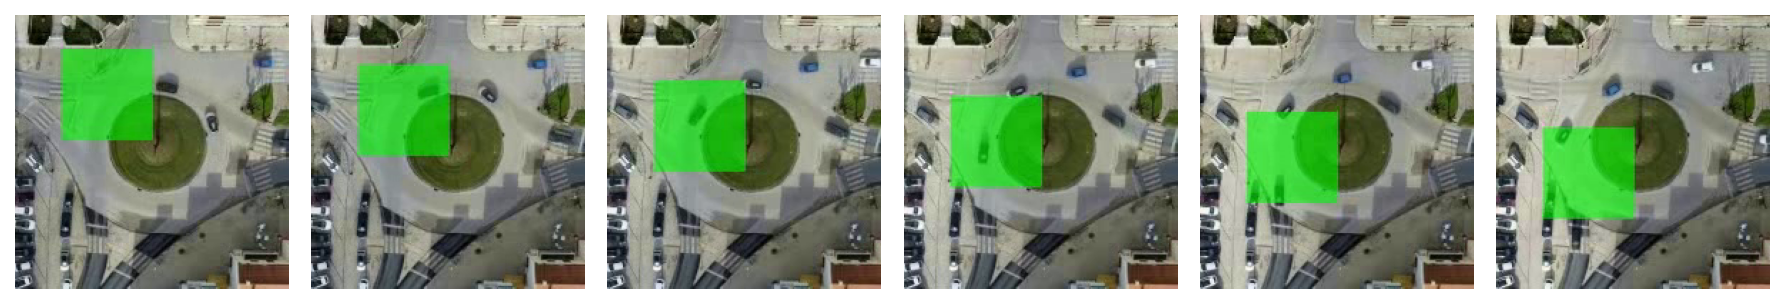
\includegraphics[width=\textwidth]{figures/13269_task_only.pdf}
\caption[An example inpainting task from our Traffic-Scenes dataset.]{An example inpainting task from our Traffic-Scenes dataset. }
\label{fig:semantics}
\end{figure*}
Further, prior work has overlooked the utility of the \emph{semantic} content of the video being inpainted, an understanding of which is particularly important for tasks where inpainting effectively amounts to inferring the behavior of occluded objects. To illustrate this, consider \Cref{fig:semantics}. The black car at the top of the roundabout enters the masked region (shown in green) shortly after the first frame, and emerges some seconds later near the bottom of the frame. For an inpainting to be plausible, the car must follow a realistic trajectory around the roundabout. Note that, without a strong prior, there is insufficient information in the context to determine what such a trajectory might look like; the model must have some notion of what makes a vehicle trajectory plausible at a semantic level. For the roundabout example above, this includes, for instance, that vehicles should remain on the road surface, that vehicles travel forward with respect to their orientation, \etc. To accomplish this, the model must also correctly observe the entry and exit points of the vehicle, which could be arbitrarily far apart from each other in the general case. Additionally, the video inpainting problem is ill-posed -- given the events observed in the context, there exists a diversity of plausible trajectories the car could take, and video inpainting methods should account for this. As such, we assert that video inpainting methods must be capable of incorporating semantic knowledge, modeling long-range dependencies, and generating diverse solutions to solve the general video inpainting problem.

 
We argue that a sensible approach to video inpainting is to learn a conditional distribution over possible inpaintings given the observed context. Indeed, generative approaches to image inpainting using GANs \citep{imin3, imin4, imin5}, autoregressive models \citep{imin1}, and diffusion models \citep{palette, repaint} have long been amongst the top performing methods for image inpainting, and are capable of generating diverse, semantically coherent outputs. Such an approach has recently been made possible by the development of diffusion models for video \citep{didrik, fdm, vdm, yang2022diffusion, voleti2022MCVD}, which are capable of generating long, temporally coherent, photorealistic samples. In this thesis, we present a framework for using conditional video diffusion models for video inpainting. We demonstrate how to use long-range temporal attention to generate semantically consistent behaviour of inpainted objects over long time horizons, even when our model cannot be jointly model all frames due to memory constraints. We can do this even for inpainted objects that have limited or no visibility in the context, a quality not present in the current literature. We report strong experimental results on several challenging video inpainting tasks, outperforming state-of-the-art approaches on a range of standard metrics.

\begin{figure*}[h!]
    \centering
    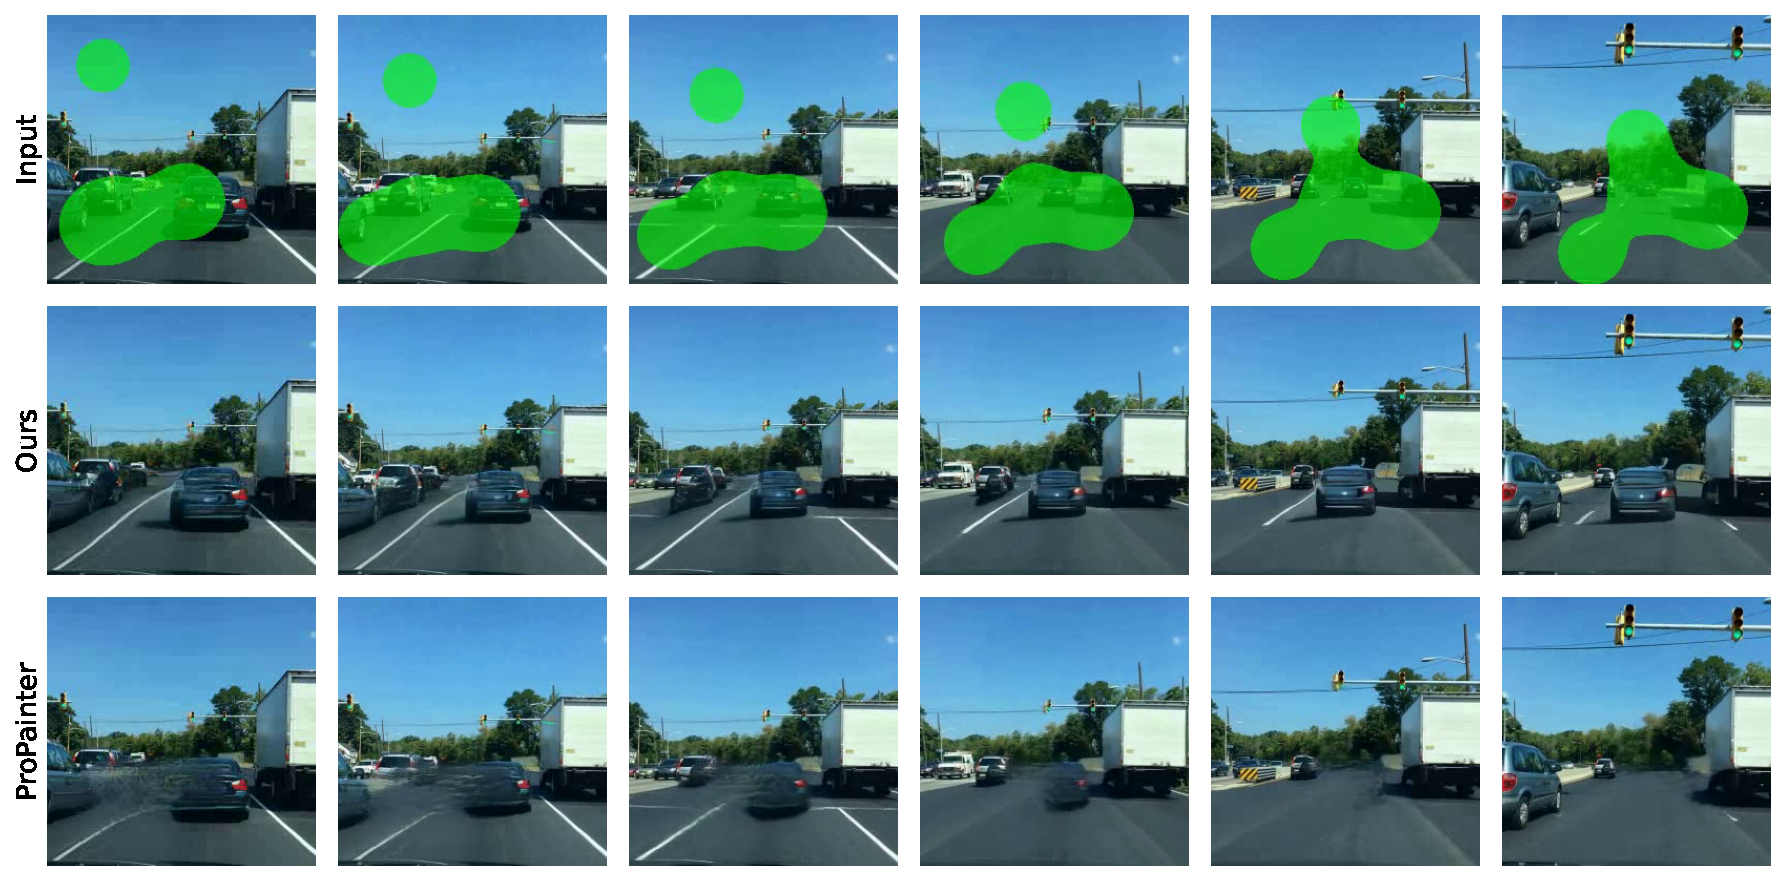
\includegraphics[width=\textwidth]{figures/bddv2.pdf}
    \caption[Inpainting results on a task from our BDD-Inpainting dataset.]{Inpainting results on a task from our BDD-Inpainting dataset. The first row shows the input to the model, with the occlusion mask marked in green. Our method (second row) is capable of generating a plausible completion of the partly occluded vehicle and realistically propagating it through time. On the contrary, in the result from the best-competing method, ProPainter \citep{propainter} (third row), the inpainted vehicle quickly fades away and is not modeled in a semantically consistent manner.}
    \label{fig:fig1}
\end{figure*}

